The statistical interpretation of the extracted distribution from events of simulation and data enables the possibility to make a statement about \gls{LFV} in nature. For the interpretation of data and simulation two hypotheses are made: the background only hypothesis (no \gls{LFV} in nature) and the signal + background hypothesis (\gls{LFV} occur in nature). In this analysis the evaluation of the hypotheses  is done with the $CL_s$ method \cite{CLS}, which is recommended by the \gls{CMS} collaboration. 

\section{Maximum likelihood approach and the $CL_s$ method}
\label{sec:section_5_1}

The measured value of a physical quantity is a random variable, which distribution can be described by probability densities. For a counting experiment the number $n$ of counted events for a specific value of the physical quantity is described by the Poisson distribution $p(n) = \frac{\lambda^{n}}{n!}e^{-\lambda}$ with $\lambda$ as the expected value of the counted events. For the case $n$ is measured in the experiment and $\lambda$ is unknown the probability density is called likelihood function $\mathcal{L}$ \cite{LIKELIHOOD}. For this analysis, which is a multi-bin counting experiment, the Poisson distributed likelihood function is defined as

\begin{equation}
	\label{eq:eq_5_1}
	\mathcal{L}(\text{data} | \mu, \vec{\theta}) = \Pi_{i} \frac{(\mu s_i+ b_i)^{n_i}}{n_i!} e^{-\mu s_i +b_i} \cdot p(\vec{\theta_i}).
\end{equation}

The first term is the Poisson distribution, where the expected bin content $i$ is parametrized with $s$ signal events and $b$ background events and a floating signal strength parameter $\mu$. This signal strength is $\mu = 0$ for the background hypothesis and $\mu>0$ for the signal + background hypothesis. Systematic uncertainties are parametrized by the floating parameter vector $\vec{\theta}$ and are described by the prior function $p$.  \\

To evaluate the experiment, the so-called test statistic $\tilde{q}_{\mu}$ is defined like 

\begin{equation}
	\label{eq:eq_5_2}
	\tilde{q}_{\mu} = -2\ln{\frac{\mathcal{L}(\text{data} | \mu, \hat{\vec{\theta_{\mu}}})}{\mathcal{L}(\text{data} | \hat{\mu}, \hat{\vec{\theta}})}}
\end{equation}

with $\mathcal{L}(\text{data} | \hat{\mu}, \hat{\vec{\theta}})$ as the global maximum of the likelihood function and $\mathcal{L}(\text{data} | \mu, \hat{\vec{\theta_{\mu}}})$ as the likelihood function, where the nuisance parameters $\hat{\vec{\theta_{\mu}}}$ are tuned to maximize the likelihood in dependence of $\mu$. For the evaluation of the hypotheses the p-values are calculated for both hypotheses. The p-values quantify the probability to find a $\tilde{q}_{\mu} > \tilde{q}_{\mu}^{obs}$ for a given value of $\mu$, where $\tilde{q}_{\mu}$ is distributed according to a probability density $f(\tilde{q}_{\mu})$, and can be calculated using

\begin{equation}
	\label{eq:eq_5_3}
	p_{\mu} = P(\tilde{q}_{\mu} > \tilde{q}_{\mu}^{obs}) = \int_{\tilde{q}_{\mu}^{obs}}^{\infty} f(\tilde{q}_{\mu}) d\tilde{q}_{\mu}.
\end{equation}

For the background hypotheses with $\mu = 0$ the p-value is defined like $p_b = p_{\mu = 0}$ and for the signal + background hypotheses with $\mu>0$ the p-value is defined like $p_s = p_{\mu>0}$. From the ratio of the p-values, the $CL_s$ classifier is defined like

\begin{equation}
	\label{eq:eq_5_4}
	CL_s = \frac{p_s}{p_b}
\end{equation}

and can used for the evaluation of the hypotheses. For a given $\mu$, demanding for example $CL_{s} < \alpha$, the signal hypotheses can be excluded with a $1-\alpha$ confidence level. To make a statement about the values of $\mu$, it is common to demand $CL_{s} < 0.05$ and tune $\mu$ until this value is reached. This value of $\mu_{CL_s = 0.05}$ and all values above can then be excluded with a confidence level of 95\%.

\section{Interpretation of the analysis}
\label{sec:section_5_2}

In this analysis the \gls{BDT} score, which is discussed in section \ref{sec:section_3_5}, is used as the discriminating variable for the counting experiment. The \gls{BDT} score is analyzed in bins of three categories, which are described in section \ref{sec:section_3_2_3}. As nuisance parameter $\vec{\theta}$ the systematic uncertainties discussed in section \ref{sec:section_4} are used.\\

The analysis is interpreted in terms of the expected limit on the signal strength $\mu_{exp}$. The calculation of $\mu_{exp}$ follows the description of section \ref{sec:section_5_1} for $\mu_{CL_s = 0.05}$, but instead of evaluating data events, an Asimov data set \cite{ASIMOV} is used. The Asimov data set is a toy data set generated with the model expectation for a given $\mu$ and the nuisance parameter $\vec{\theta}$. In this case the Asimov data set is generated for the background-only hypothesis with $\mu = 0$. The expected limit quantifies the power of the analysis of setting the constraint on the signal strength, if the background only hypotheses is realized. \\

The constraint on the signal strength can be translated into a constraint on the $\text{BR}(Z\to\text{LFV})$ with $\text{LFV} \in (e\mu, e\tau, \mu\tau)$. In the signal expectation $s$, according to equation \ref{eq:eq_3_3}, the limit on the branching ratios of previous analysis is used. Setting a constraint on the signal strength $\mu$ also set a constraint on the signal expectation $s$. So the expected limit on the branching ratio $\text{BR}_{exp}(Z\to\text{LFV})$ is related to the expected limit on the signal strength $\mu_{exp}$ via 

\begin{equation}
	\text{BR}(Z\to\text{LFV}) \cdot \mu_{exp} > \text{BR}_{exp}(Z\to\text{LFV})
\end{equation}

This relation can now be evaluated to judge the sensitivity of the analysis compared to the previous analysis, which set constraints on the branching ratio. For $\mu_{exp} > 1$ the expected branching ratio is not as good as the constraints from the previous analysis, the sensitivity of the previous analysis is not reached yet. For $\mu_{exp} < 1$ the expected limit gives a better constraint on the branching ration compared to the previous analysis, a gain in sensitivity is achieved. 


\section{Results}
\label{sec:section_5_3}

The results of this analysis are given in terms of expected limits on the branching ratio $\text{BR}(Z\to\text{LFV})$ for each final state. \\

The figure \ref{fig:fig_5_1} shows the excepted limits in each category and the combination of all categories. Generally the sensitivity increases for lower jet multiplicity. This is expected, because as shown in the distribution in figure \ref{fig:fig_3_7}, the signal to background ratio gets worse for higher jet multiplicity. In the $e\mu$ final state the change in sensitivity for each category in comparison to the $e\tau$ and $\mu\tau$ final state can be explained with the dominant $t\bar{t}$ background in the multi-jet category for $e\mu$. \\

Also the latest observed limit is shown in comparison to the combined expected limit of this analysis. In the $e\mu$ final state the expected limits give a three times better constraint on the branching ratio than the latest observed limit. And because the latest observed limits lie far above the uncertainty bands of the expected limit of this analysis, a possible excess due to a \gls{LFV} signal could be measured. This gain in sensitivity is expected, because the latest observed limit was measured during the \gls{CMS} Run I with a lower integrated luminosity of $\mathcal{L}_{int} = 19.8$ fb$^{-1}$ compared to the integrated $\mathcal{L}_{int} = 36.9$ fb$^{-1}$ of this analysis. For the $e\tau$ and $\mu\tau$ final state the expected limits on the branching are almost as good, respectively as good as the constraint given by previous analysis. That the limits are not better like in the $e\mu$ final state, can be explained by the fact, that the latest observed limits in this final state were measured with data of the electron-positron collider \gls{LEP}. In an electron-positron collider the initial state of all processes is known, in the case of proton-proton collisions \gls{PDF} have to be used as described in section \ref{sec:section_2_1_2}. With leptons as colliding objects, the \gls{QCD} multi-jet background was not an issue at \gls{LEP}, which gives a much clearer background compared to proton-proton collider. The analysis of the \gls{TAUH} is therefore much more challenging at \gls{LHC}. 

\begin{figure}[htp]
	\centering
	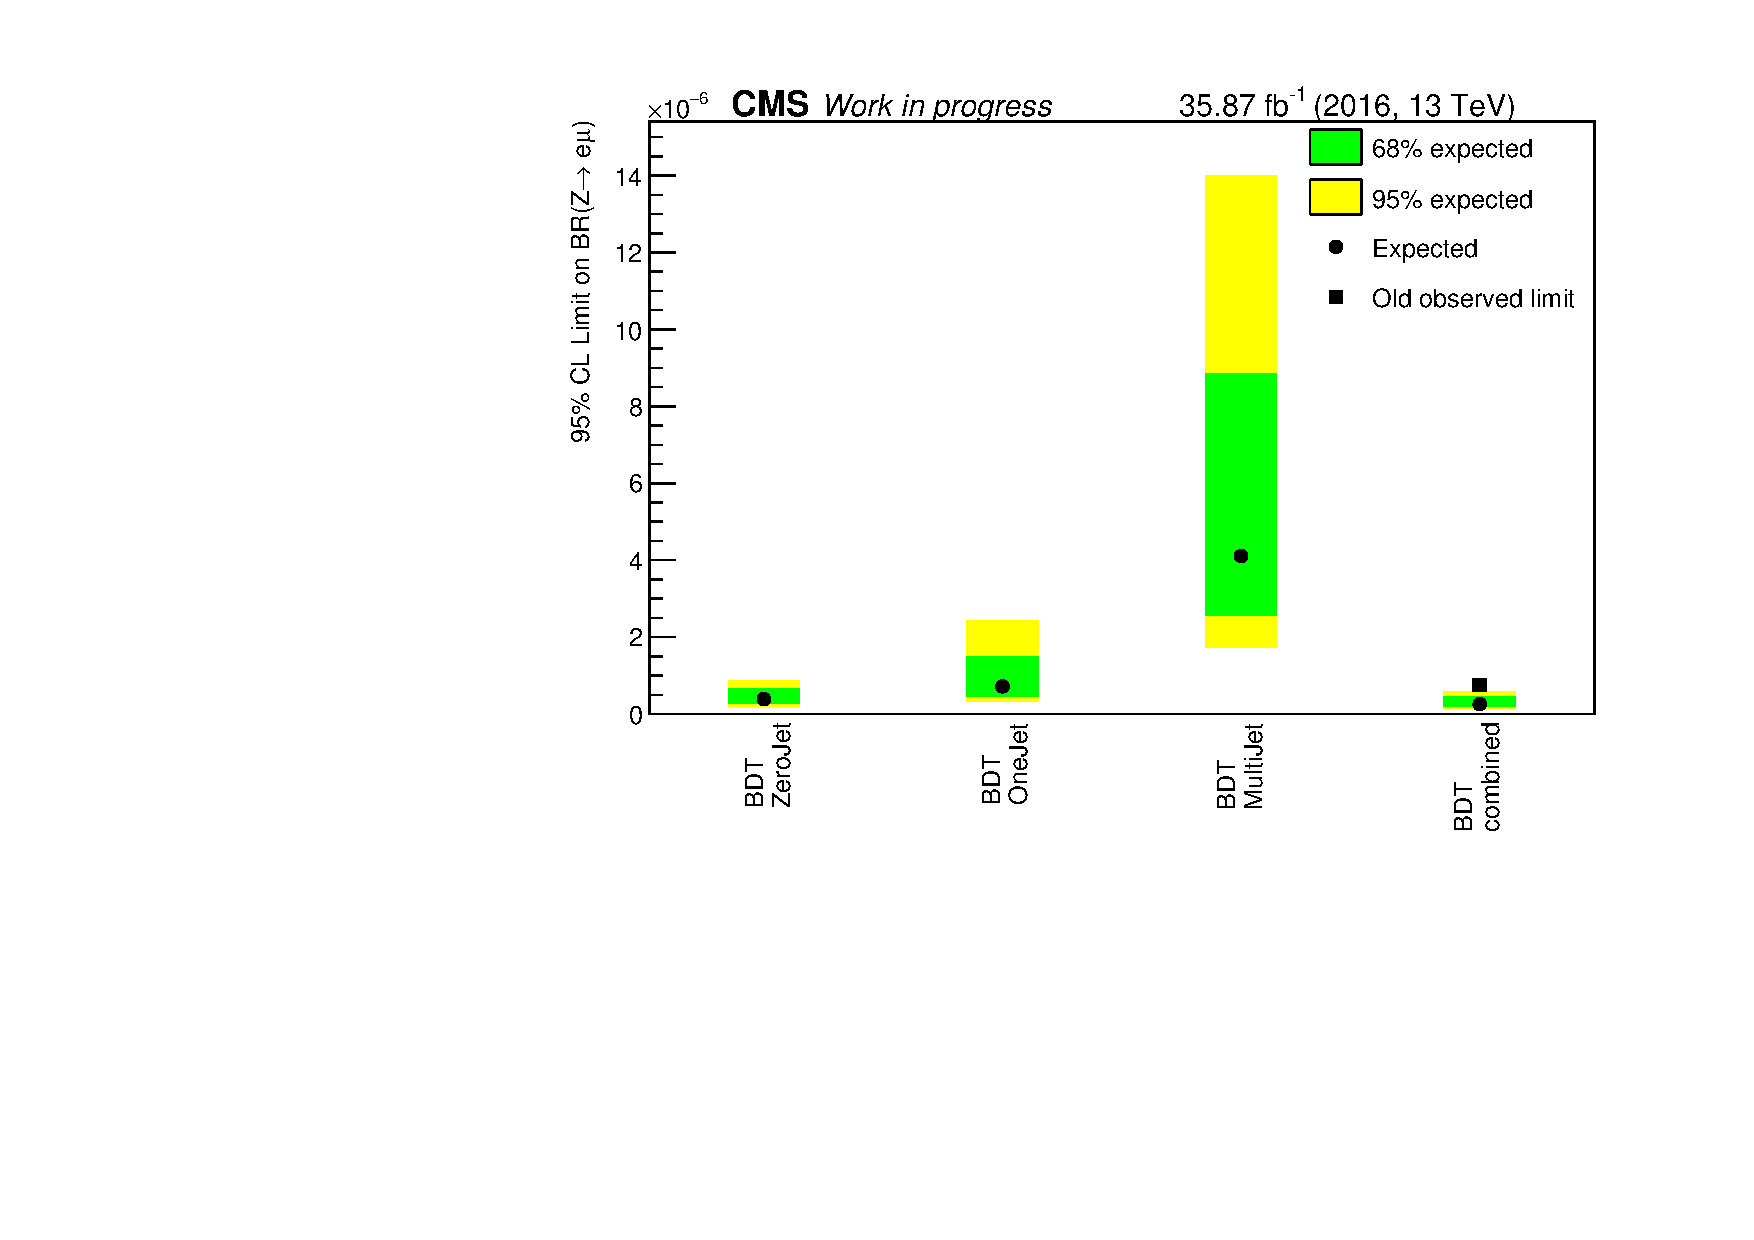
\includegraphics[width=0.6\textwidth]{plots/em/limits.pdf}
	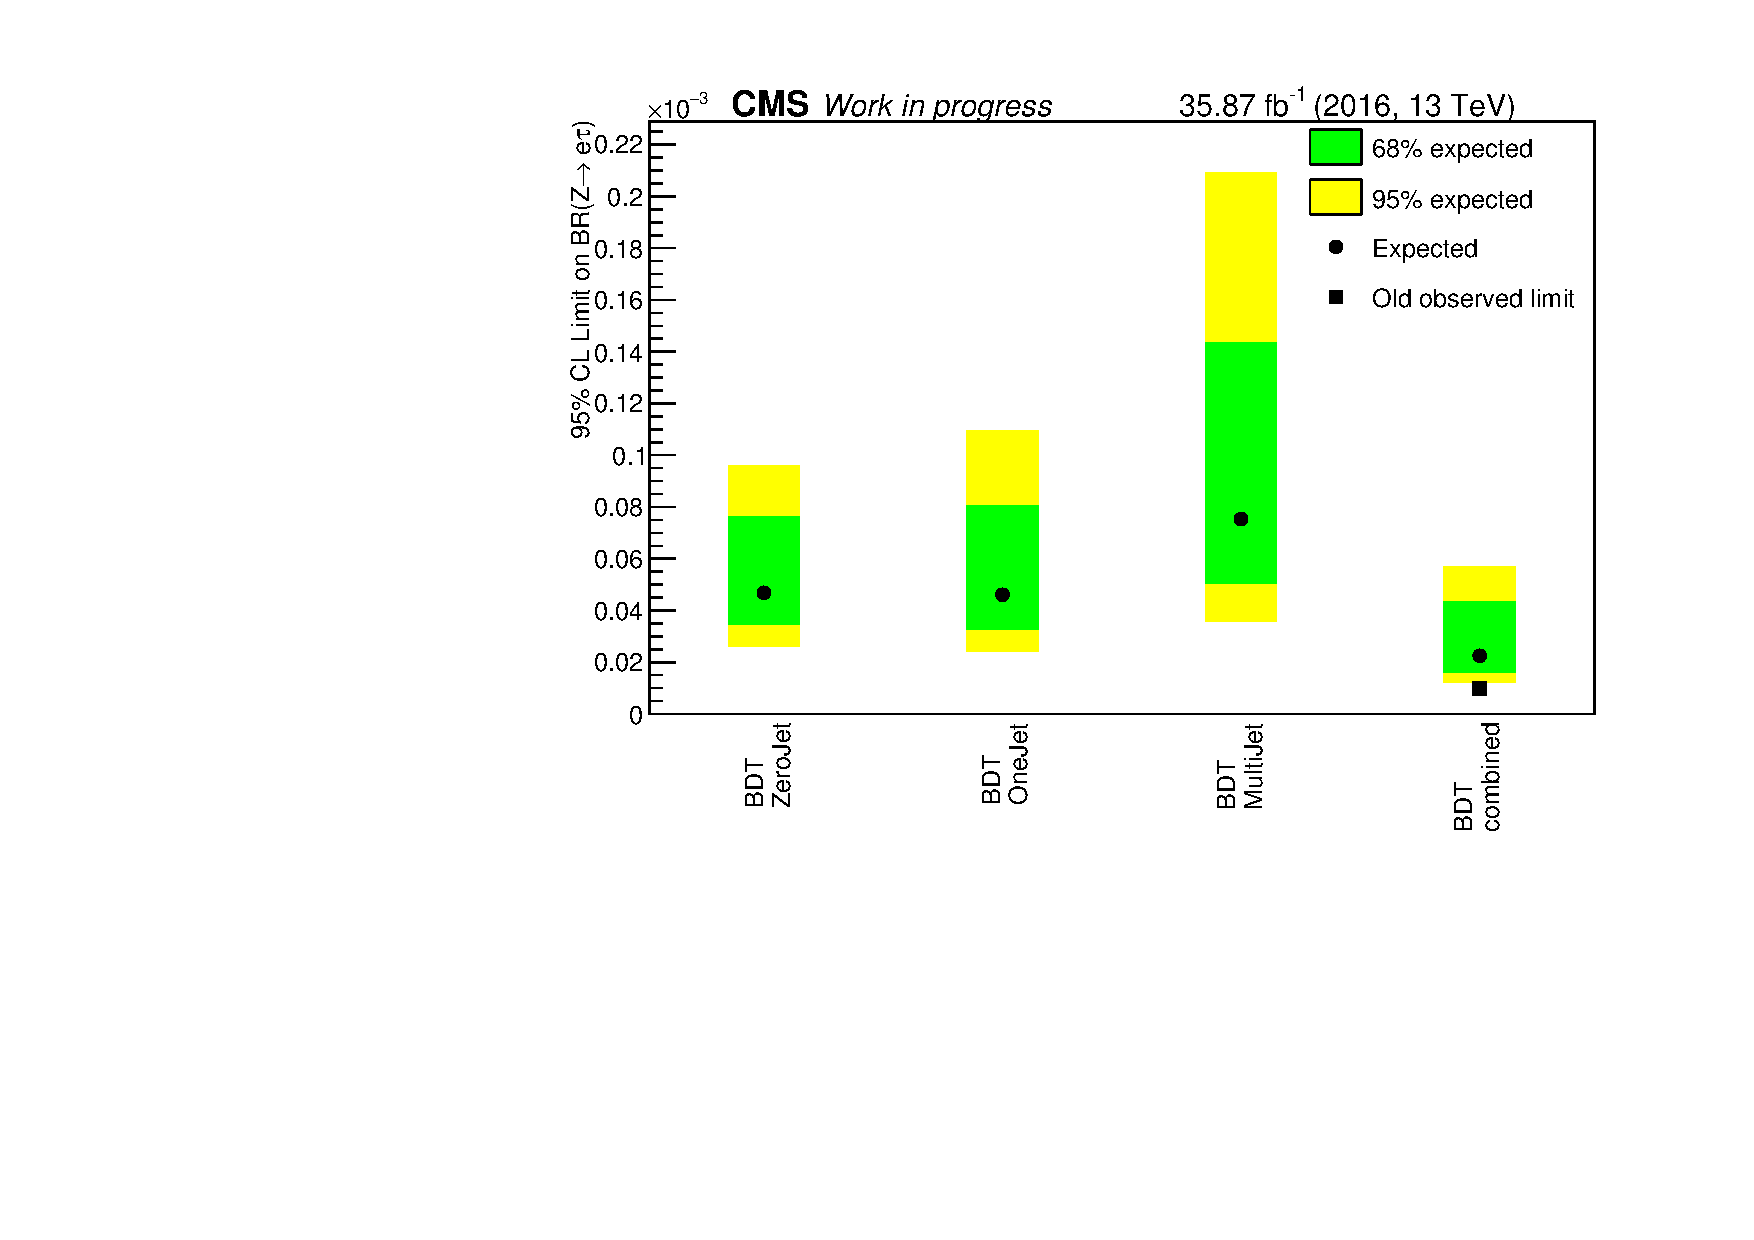
\includegraphics[width=0.6\textwidth]{plots/et/limits.pdf}
	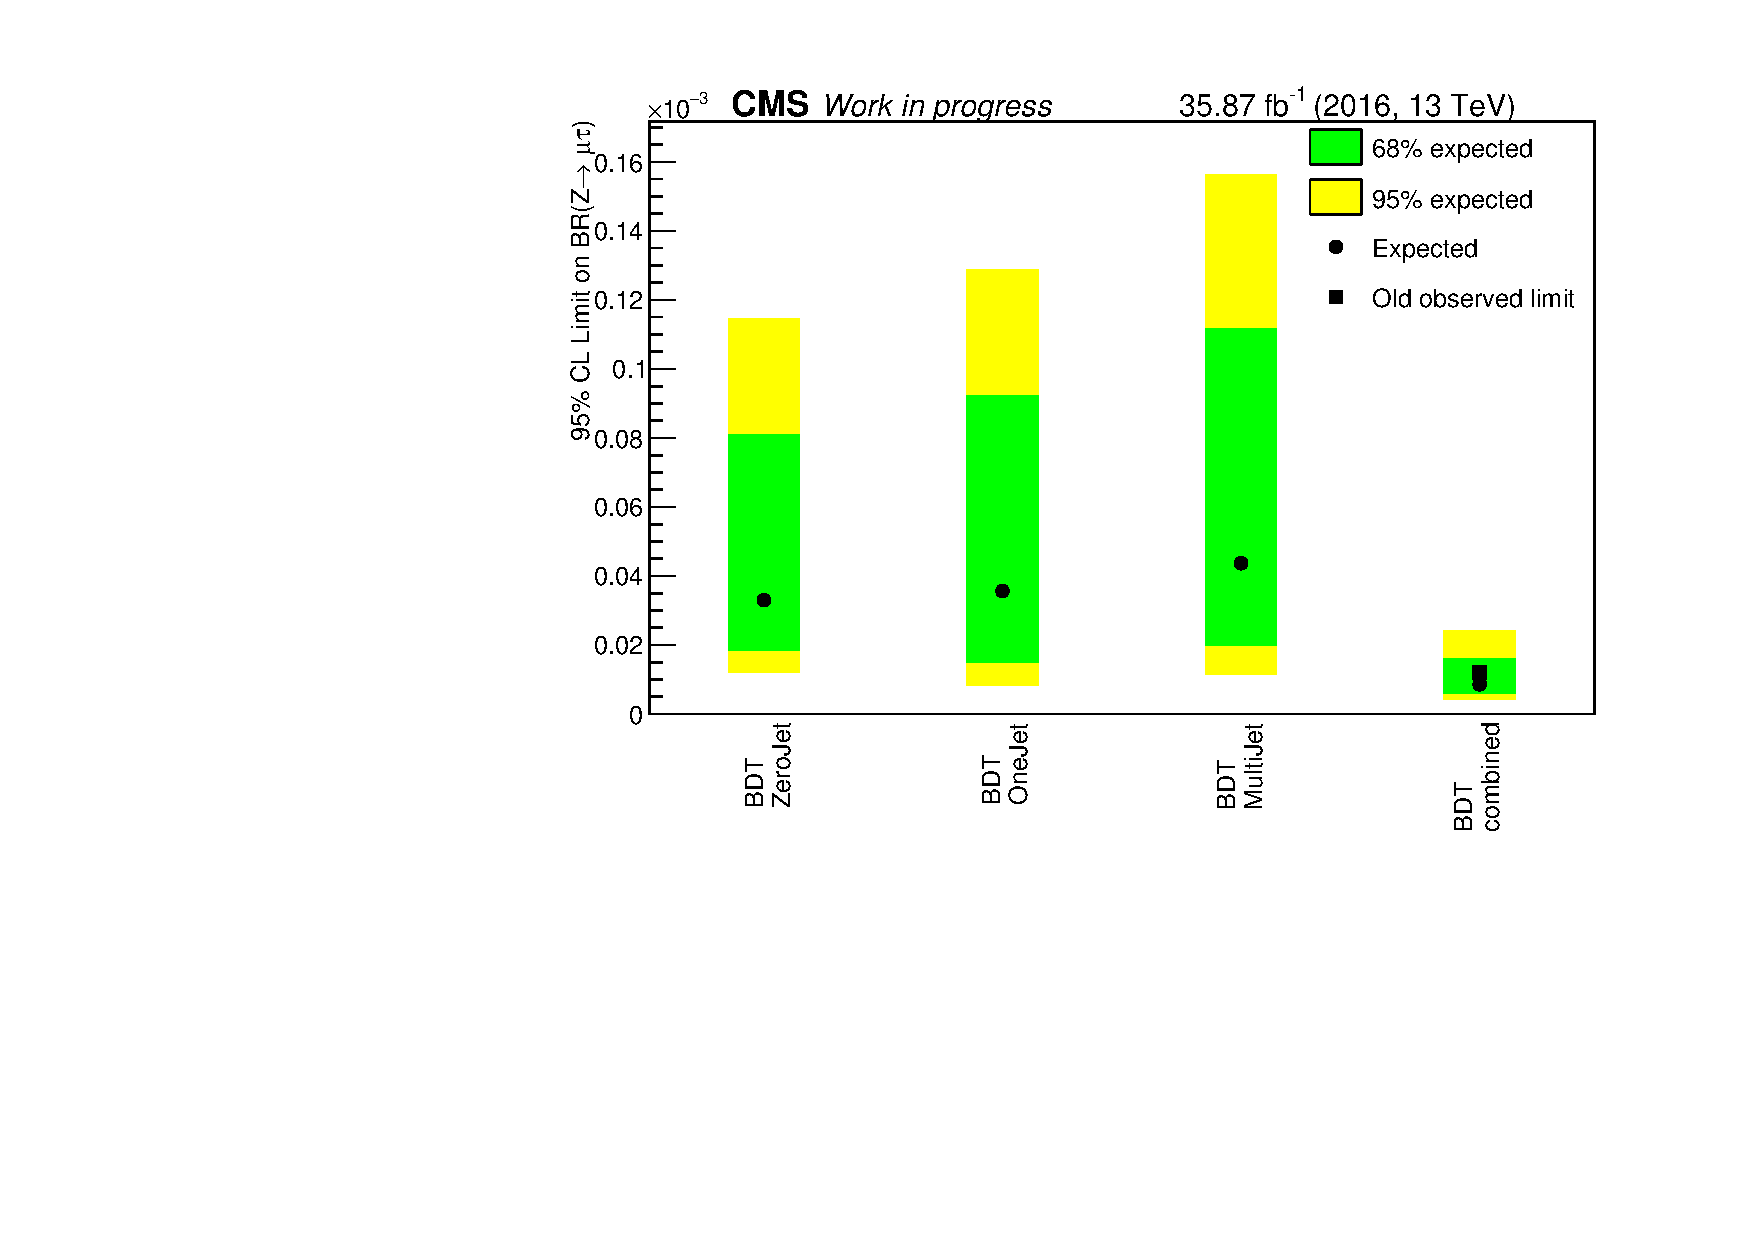
\includegraphics[width=0.6\textwidth]{plots/mt/limits.pdf}

	\caption[Expected limits on the branching ratios]{Expected limits on the branching ratio $\text{BR}(Z\to\text{LFV})$ for each final state. The limits are given for all three categories and the combination of all of them, together with the one/two sigma uncertainty.}
	\label{fig:fig_5_1}
\end{figure}
















